%%% Local Variables:
%%% TeX-command-extra-options: "-shell-escape"
%%% mode: latex
%%% TeX-master: t
%%% End:
\documentclass{beamer}
\usepackage{caption}
\usepackage{minted}
\usepackage{tikz}
\usetikzlibrary{shapes.geometric, arrows}
\tikzstyle{startstop} = [rectangle, rounded corners, minimum width=3cm, minimum height=1cm,text centered, draw=black, fill=red!30]
\tikzstyle{io} = [trapezium, trapezium left angle=70, trapezium right angle=110, minimum width=1.5cm, minimum height=0.6cm, text centered, draw=black, fill=blue!30]
\tikzstyle{process} = [rectangle, minimum width=1.5cm, minimum height=0.5cm, text centered, draw=black, fill=orange!30]
\tikzstyle{decision} = [circle, radius=2.5cm, text centered, draw=black, fill=green!30]
\tikzstyle{arrow} = [thick,->,>=stealth]
\usepackage[labelformat=simple]{subcaption}

\usetheme{Singapore}
\title{Lecture 3}
%\subtitle{in Racket}
%\author{Peter Campora}
%\institute{ULL}
%\date{\today}

%This lectures introduces Racket basics and the right way to program
\begin{document}
\begin{frame}
\titlepage
\end{frame}

\section{Arithmetic in Racket}
\begin{frame}
  \frametitle{Arithmetic Revisited}
  Warning! The start of this lecture will be a bit boring since it introduces
  the basic elements of Racket--starting with how to do arithmetic.
  \begin{itemize}
  \item<2-> \mintinline{Scheme}{(+ 1 1)}
  \item<3-> Evaluate inner parentheses first: \mintinline{Scheme}{(+ 1 (+ 1 (+ 1 1) 2) 3 4 5)}
  \item<4-> == \mintinline{Scheme}{(+ 1 (+ 1 2 2) 3 4 5)}
  \item<5-> == \mintinline{Scheme}{(+ 1 5 3 4 5)}
  \item<6-> == \mintinline{Scheme}{(+ 1 5 3 4 5)}
  \item<7-> == \mintinline{Scheme}{(+ 1 (+ 1 2 2) 3 4 5)}
  \end{itemize}
\end{frame}

\begin{frame}
  \frametitle{Arithmetic Revisited (cont)}
  \begin{itemize}
  \item<1-> Primitive form is \mintinline{Scheme}{(operator [number...])}
  \item<2-> A list of useful operators:  +, -, *, /, abs, add1, ceiling, denominator, expt, floor, gcd, log, max, numerator, quotient, random, remainder, sqr, and tan
  \item<3-> Racket has an extensive \emph{numeric tower}.
  \item<4-> What would \mintinline{Scheme}{(/ 4 3)} produce in Java?
  \item<5-> Instead of producing a float, it produces $\frac{4}{3}$.
  \item<6-> To get a float, you need to use \mintinline{Scheme}{(exact->inexact (/ 4 3))}
  \item<7-> Other operations like \mintinline{Scheme}{(sqrt 2)} immediately produce floats.
  \item<8-> Let's play around with this a bit!
  \end{itemize}
\end{frame}

\begin{frame}
  \frametitle{Arithmetic of Strings}
  You may think of arithmetic involving integers or real numbers, but
  we can also have arithmetic on strings!
  \begin{itemize}
  \item<2-> String concatenation is our basic operation: \mintinline{Scheme}{(string-append "Hello " "World")}
  \item<3-> We can give it multiple arguments: \mintinline{Scheme}{(string-append "What a " "lovely " "day" " for Racket!")}
  \item<4-> The identity element for string-append is "":
    \mintinline{Scheme}{(string-append "foo" "")}
  \item<5-> We can get the length of strings: \mintinline{Scheme}{(string-length "abc")}
  \item<6-> We can extract a specific character: \mintinline{Scheme}{(string-ref "abc" 0)}
  \item<7-> We can take a substring of a string: \mintinline{Scheme}{(substring "foobar" 0 3)}
  \item<8-> Can convert numbers to strings: \mintinline{Scheme}{(number->string 42)}
  \end{itemize}
\end{frame}

\begin{frame}
  \frametitle{Arithmetic of Images}
  A lot of functions are available for manipulating images:
  \begin{itemize}
  \item<2-> Circles: \mintinline{Scheme}{(define my-circle (circle 10 "outline" "green"))}
  \item<3-> Rectangles: \mintinline{Scheme}{(define my-rectangle (rectangle 10 20 "solid" "red"))}
  \item<4-> Get the height of an image: \mintinline{Scheme}{(image-height my-rectangle))}
  \item<5-> Or the width: \mintinline{Scheme}{(image-height my-rectangle))}
  \item<6-> You can layer images with overlay: \mintinline{Scheme}{(overlay my-circle my-rectangle)}
  \item<7-> See also \mintinline{Scheme}{overlay/xy} and \mintinline{Scheme}{overlay/align}
  \end{itemize}
\end{frame}

\begin{frame}
  \frametitle{Arithmetic of Images (cont.)}
  The starting points for drawing images typically involves the functions below:
  \begin{itemize}
  \item<2-> \mintinline{Scheme}{empty-scene}, \mintinline{Scheme}{place-image},
    and \mintinline{Scheme}{scene+line}
  \item<3-> To create an empty-scene:
    \mintinline{Scheme}{(define canvas (empty-scene 100 100 "white"))}
  \item<4-> To place an image into the scene:
    \mintinline{Scheme}{(place-image my-rectangle 50 50 canvas)}  
  \item<5-> Copy this image into Dr. Racket: 
\includegraphics[width=0.05\textwidth]{images/cat.png}    
  \end{itemize}
\end{frame}

\begin{frame}
  \frametitle{Arithmetic Laws}
  \begin{center}
    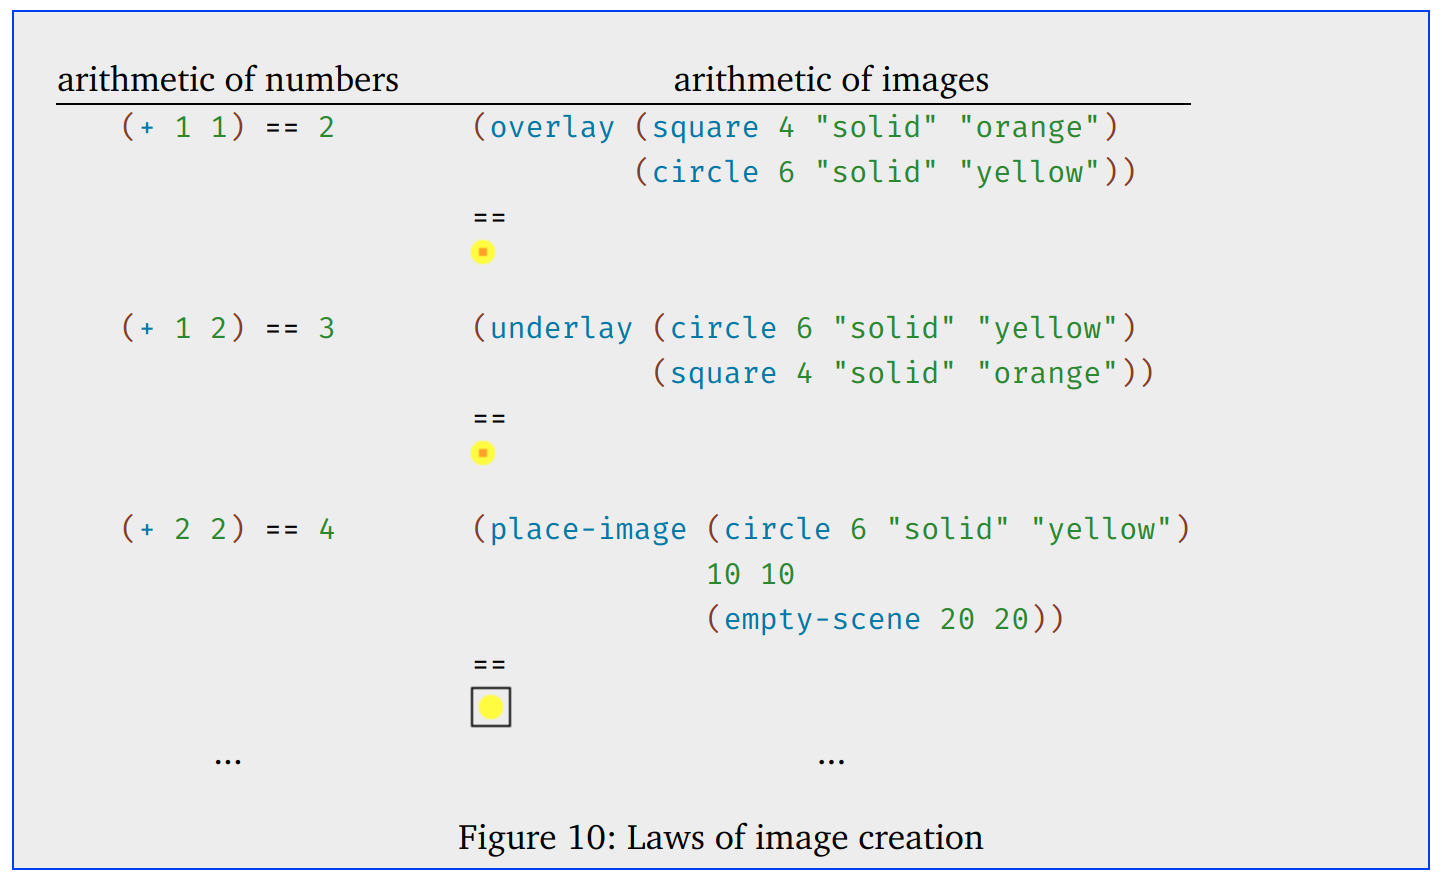
\includegraphics[width=0.7\textwidth]{images/Arithmetic-Images.png}
  \end{center}
\end{frame}

% \defverbatim[colored]\schemeTrue{
% \begin{minted}{Scheme}
%   #t
% \end{minted}
% }

\defverbatim[colored]\cond{
\begin{minted}{Scheme}
    (cond 
      [(> x 0) 1]
      [(= x 0) 0]
      [else -1])
\end{minted}
}

\begin{frame}
  \frametitle{Arithmetic of Booleans}
  Boolean Arithmetic should look familiar to all of you.
  \begin{itemize}
  \item<2-> The primitive boolean values are: 
    \text{\#t} and \text{\#f}
  \item<3-> The functions \mintinline{Scheme}{and}, \mintinline{Scheme}{or}, and
    \mintinline{Scheme}{not} do exactly what you expect
  \item<4-> We can write conditional expressions with the form:
    \mintinline{Scheme}{(if test-exp true-branch else-branch)}
  \item<5-> What does the following expression evaluate to?
    \mintinline{Scheme}{(+ 1 (if (< 0 1) 1 2))}
  \item<6-> When we have more conditions we use \mintinline{Scheme}{cond}:
    \cond
  \end{itemize}  
\end{frame}

\defverbatim[colored]\catProgram{
\begin{minted}{Scheme}
    (define cat-height (image-height cat))
    (define cat-width (image-width cat))
    
    (if (>= cat-height cat-width) 
        "long cat!" 
        "heckin chonker!")
\end{minted}
}

\begin{frame}
  \frametitle{Our First Program}
  Let's write a program to classify whether this cat is a long cat or a heckin
  chonker!
  \begin{center}
    
\includegraphics[width=0.1\textwidth]{images/cat.png}    
  \end{center}
  \begin{itemize}
  \item<2-> It should be a long cat if its height (tail height counts) is higher
    than its width.
  \item<3-> Help me write it! We're going to need
    \mintinline{Scheme}{image-height} and \mintinline{Scheme}{image-width}.
  \item<4-> Here it is: \catProgram
  \end{itemize}
\end{frame}

\begin{frame}
  \frametitle{Predicates}
  Predicates are a short way of saying boolean valued function. Let's take
  a look at some important predicates in Racket.
  \begin{itemize}
  \item<2-> We can check if something is a number with \mintinline{Scheme}{number?}
  \item<3-> \mintinline{Scheme}{(number? 2)}, \mintinline{Scheme}{(number? 2.3)}, and \mintinline{Scheme}{(number? 2/3)} all return true
  \item<4-> Surprisingly \mintinline{Scheme}{(rational? 2)}, \mintinline{Scheme}{(rational? (sqrt 2))}, and \mintinline{Scheme}{(rational? 2/3)} all return true too. 
  \item<5-> Use \mintinline{Scheme}{(exact? (sqrt 2))} or \mintinline{Scheme}{(inexact? (sqrt 2))}
  \item<6-> There are many other predicates: \mintinline{Scheme}{real?},
    \mintinline{Scheme}{boolean?}, \mintinline{Scheme}{image?},
    \mintinline{Scheme}{string?}, \mintinline{Scheme}{complex?}, ...
  \end{itemize}
\end{frame}

\defverbatim[colored]\predicateSkeleton{
\begin{minted}{Scheme}
    (cond
      [(... in) ...]
      ...)
\end{minted}
}

\defverbatim[colored]\predicatePartial{
\begin{minted}{Scheme}
    (cond
      [(string? in) ...]
      ...)
\end{minted}
}
\defverbatim[colored]\predicateFinal{
\begin{minted}[fontsize=\footnotesize]{Scheme}
    (cond 
        [(string? in) (string-length in)]
    	[(and (number? in) (> in 0)) (sub1 in)]
    	[(image? in) (* (image-height in) (image-width in))]
    	[else in])
\end{minted}
}
\begin{frame}
  \frametitle{Programming With Predicates}
  Create an expression that converts the value of \mintinline{Scheme}{in} to a positive number. For a String, it determines how long the String is; for an Image, it uses the area; for a Number, it decrements the number by 1, unless it is already 0 or negative; for true it uses 10 and for false 20.
\begin{itemize}
\item<2-> Let's diagram this out.
\item<3-> Here is our skeleton: \predicateSkeleton
%\item<4-> \predicatePartial
\item<4-> Here is our final version: \predicateFinal
\end{itemize}

\end{frame}

% \begin{frame}
%   \frametitle{Booleans and Conditionals}
%   \begin{itemize}
%   \item<2-> The structure of basic conditional statements:
%     \mintinline{Scheme}{(if test-exp true-branch else-branch)}
%   \item<3-> \mintinline{Scheme}{(if #t 1 2) ;;produces 1}
%   \item<4-> Can use it as an argument to other operations:
%     \mintinline{Scheme}{(+ 1 (if #t 1 2))}
%   \item<5-> This means that conditionals in Racket are expressions.
%   \item<6-> If we don't want to nest if-expressions, we use \mintinline{Scheme}{cond}
%   \item<7-> \mintinline{Scheme}{(cond [test-1 result-1] ...[test-n result-n])}
%   \item<8-> Let's record the sign of some integer x: \cond
%   \end{itemize}
% \end{frame}


\section{From Arithmetic to Functions}
\begin{frame}
  \frametitle{Our Bread and Butter}
  \begin{center}
    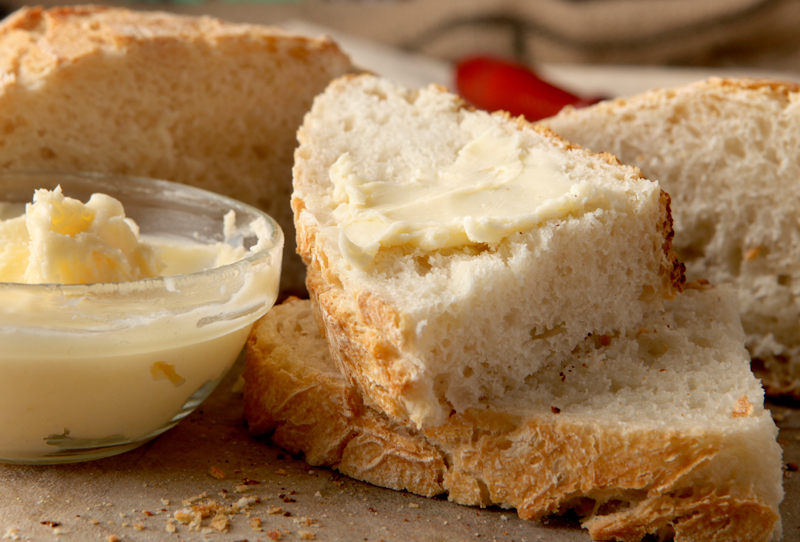
\includegraphics[width=0.4\textwidth]{images/bread-butter.jpg}
  \end{center}
  \begin{itemize}
  \item<2-> Yum!
  \item<3-> Functions are the bread and butter of functional programming, so let's get that bread!
  \item<4-> \huge But first, what is a function?
  \end{itemize}
\end{frame}



\begin{frame}
  \frametitle{The Algebra of Programming}
  \begin{figure}
    \begin{subfigure}{0.45\textwidth}
      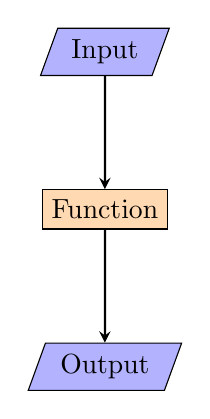
\begin{tikzpicture}[node distance=2cm]
        % \node (start) [startstop] {Start};
        \node (in1) [io] {Input};
        \node (pro1) [process, below of=in1] {Function};
        \node (out1) [io, below of=pro1] {Output};
        \draw [arrow] (in1) -- (pro1);
        \draw [arrow] (pro1) -- (out1);
      \end{tikzpicture}
    \end{subfigure}
    \pause
    \begin{subfigure}{0.45\textwidth}
      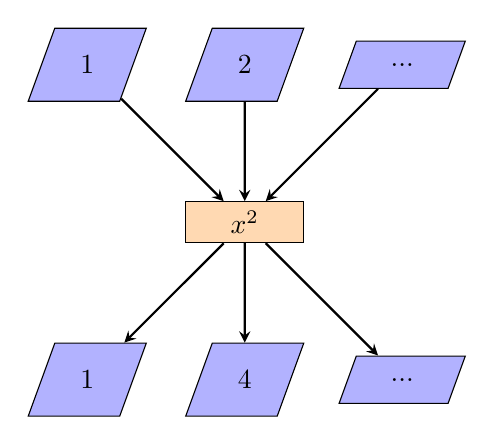
\begin{tikzpicture}[node distance=2cm]
        % \node (start) [startstop] {Start};
        \node (in1) [io] {2};        
        \node (in2) [io, right of=in1] {...};
        \node (in3) [io, left of=in1] {1};
        \node (pro1) [process, below of=in1] {$x^2$};

        \node (out1) [io, below of=pro1] {4};
        \node (out2) [io, right of=out1] {...};
        \node (out3) [io, left of=out1] {1};
        
        \draw [arrow] (in1) -- (pro1);
        \draw [arrow] (in2) -- (pro1);
        \draw [arrow] (in3) -- (pro1);
        
        \draw [arrow] (pro1) -- (out1);
        \draw [arrow] (pro1) -- (out2);
        \draw [arrow] (pro1) -- (out3);
      \end{tikzpicture}
    \end{subfigure}
  \end{figure}
\end{frame}

\defverbatim[colored]\arrayList{
\begin{minted}{Java}
import java.util.ArrayList;
class Main {
  public static void main(String[] args) {
    System.out.println("Hello world!");
    ArrayList<Integer> alist = new ArrayList<Integer>();
    alist.add(1);
    alist.add(2);
    System.out.println(alist.remove((Object)1));
    System.out.println(alist.remove((Object)1));
  }
}
\end{minted}
}

\begin{frame}
  \frametitle{Definitions and Misconceptions}
  Mathematicians and Computer Scientists \emph{love} definitions.
  \begin{itemize}
    \item<2-> A \textbf{relation} is a set of ordered pairs.
    \item<3-> A \textbf{function} is a relation for which each value from the set the first components of the ordered pairs is associated with exactly one value from the set of second components of the ordered pair.
    \item<4-> Let's consider what isn't a function.
    \item<5-> \mintinline{Java}{aList.remove((Object)1);//assume ArrayList<Integer>}
    \item<6-> Repeatedly calling this method with the input produces
      different results.
    \item<7-> So this is a relation and not a function!
  \end{itemize}
\end{frame}

\begin{frame}
  \frametitle{A Difference in Design 1}
  Let's take a look at an idealized model of object oriented design:
  \pause
  \begin{center}
    \includegraphics[width=0.65\textwidth]{images/oo-design.png}
  \end{center}
\end{frame}

\begin{frame}
  \frametitle{A Difference in Design 2}
  Functional design is just about composing a series of functions:
  \pause
  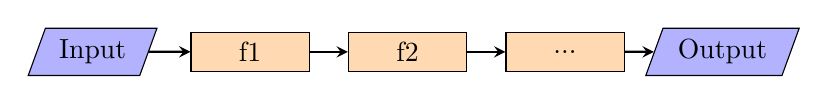
\begin{tikzpicture}[node distance=2cm]
    % \node (start) [startstop] {Start};
    \node (in1) [io] {Input};
    \node (pro1) [process, right of=in1] {f1};
    \node (pro2) [process, right of=pro1] {f2};
    
    \node (pro3) [process, right of=pro2] {...};
    \node (out1) [io, right of=pro3] {Output};
    \draw [arrow] (in1) -- (pro1);
    \draw [arrow] (pro1) -- (pro2);
    \draw [arrow] (pro2) -- (pro3);
    \draw [arrow] (pro3) -- (out1);
  \end{tikzpicture}
  \begin{itemize}
  \item<2-> Our focus is on how to model the input and output data.
  \item<3-> From there, our program is a series of functions that transform
    the input data into the output data.
  \item<4-> We carefully segregate \emph{effectful} code from our pure functions.
  \item<5-> \includegraphics[width=0.2\textwidth]{images/haskell.png}
  \end{itemize}
      
\end{frame}

\begin{frame}
  \frametitle{Getting Our Hands Dirty}
  When we defined constants in Racket, we used the form:
  \mintinline{Scheme}{(define constant exp)}
  \begin{itemize}
  \item<2-> To define functions: \mintinline{Scheme}{(define (fun-name params...) fun-body)}
  \item<3-> To define $square(x) = x^2$:
    \mintinline{Scheme}{(define (square x) (* x x))}
  \item<4-> For a function of two parameters:
    \mintinline{Scheme}{(define (add x y) (+ x y))}
  \end{itemize}
\end{frame}

\begin{frame}
  \frametitle{Debugging Incorrect Code}
  Consider the following function:
  \mintinline{Scheme}{(define (my-not b) (not b 1))}
  \begin{itemize}
  \item<2-> What happens when we make the following call? \mintinline{Scheme}{(my-not t)}
  \item<3-> \includegraphics[width=0.4\textwidth]{images/debugger.png}
  \item<4-> Let's play around with the debugger.
  \end{itemize}
\end{frame}

\begin{frame}
  \frametitle{Defining Basic Functions}
  Defining the distance to the origin $f(x, y) = \sqrt{x^2 + y^2}$ is simple:
  \begin{itemize}
  \item<2-> \mintinline{Scheme}{(define (distance x y) (sqrt (+ (sqr x) (sqr y))))}
  \item<3-> Defining implication $p \Rightarrow q$ as a function is straightforward.
  \item<4-> \mintinline{Scheme}{(define (==> p q) (or (not p) q))}
  \item<5-> Here is a secret: \mintinline{Scheme}{(f . ==> . t)}
  \item<6-> Place dots around a function to use it infix.    
  \end{itemize}
\end{frame}

\begin{frame}
  \frametitle{Designing Batch Programs}
  Often we need to write \emph{scripts} (batch program) that combine a bunch of
  function definitions into the completion of a task. This is in contrast to
  interactive or live applications that are built around some sort of event loop.
  \begin{itemize}
  \item<2-> Let's consider writing a program that fills a letter template with different names. I want to fill in the name of the person that I request the letter
    from, and the name of the company to send it to. While we're at it, let's
    make it so I can sign the letter with different names.
  \item<3-> The anatomy of a letter consists of opening, body, and closing that
    need to be parameterized by names.
  \item<4-> Let's start with the opening:
    \mintinline{Scheme}{(define (opening fst) (string-append "Dear " fst ","))}
  \end{itemize}
\end{frame}

\defverbatim[colored]\body{
\begin{minted}[fontsize=\footnotesize]{Scheme}
(define (body company)
  (string-append "I am applying for a job at " company "..."))
\end{minted}
}

\defverbatim[colored]\closing{
\begin{minted}[fontsize=\footnotesize]{Scheme}
(define (closing signature-name)
  (string-append "Sincerely," "\n\n" signature-name "\n"))
\end{minted}
}

\defverbatim[colored]\letter{
\begin{minted}[fontsize=\footnotesize]{Scheme}
(define (letter recipient company signature-name)
  (string-append
    (opening recipient)
    "\n\n"
    (body company)
    "\n\n"
    (closing signature-name)))
\end{minted}
}
\begin{frame}
  \frametitle{Our First Batch Program}
  From here, let's move onto making a function to insert a company in the body:
  \body
  \pause
  And finally, here's the closing:
  \closing
  Finally, the main ``script'' part of our program is:
  \letter
\end{frame}

\begin{frame}
  \frametitle{What about IO?}
  Our program was a pure function since it always produces the same letter
  when called with the same input. But in reality, we might want to prompt
  the user for input and display the letter as output. For now, we will just show
  how to print the letter.
  \begin{itemize}
  \item<2-> To use IO we must first add this to our program:
    \mintinline{Scheme}{(require 2htdp/batch-io)}
  \item<3-> \mintinline{Scheme}{(write-file 'stdout (letter "Mr. Campora" "WPI" "Bob Trufant"))}
  \item<4-> So in this since, our program is a call to one impure procedure after
    the composition of multiple pure functions did all of the work.
  \item<5-> One of the main goals of functional programming is to separate the
    pure core logic of the program from the effectful parts.    
  \end{itemize}
\end{frame}

\begin{frame}
  \frametitle{More About Structure}
  \begin{center}
    \includegraphics[width=0.4\textwidth]{images/FunctionalStructure.pdf}
  \end{center}
  \begin{itemize}
  \item<2-> Functional programming is about embedding a referentially transparent
    core into a layer that feeds data in and out of the stateful world.
  \item<3-> This really aids testing, as you should be able to write tests for
    the majority of the functions in the pure core. We'll discuss testing later.
  \item<4-> You should design your programs so that each piece of
    (repeatable) functionality is separated into its own function.
  \end{itemize}
\end{frame}

\begin{frame}
  \frametitle{Why Many Functions?}
  To illustrate the importance of writing many functions, let's consider
  writing a program to calculate the profit of a theater with respect to
  ticket cost and attendance.
  \pause
  \\ \\
  \textbf{Sample Problem} The owner of a monopolistic movie theater in a small town has complete freedom in setting ticket prices. The more he charges, the fewer people can afford tickets. The less he charges, the more it costs to run a show because attendance goes up. In a recent experiment the owner determined a relationship between the price of a ticket and average attendance.
  \pause
  \begin{center}
    \includegraphics[width=0.4\textwidth]{images/Monopoly.jpg}
  \end{center}
\end{frame}

\begin{frame}
  \frametitle{Making Other People Money}
  At a price of \$5.00 per ticket, 120 people attend a performance. For each 10-cent change in the ticket price, the average attendance changes by 15 people. That is, if the owner charges \$5.10, some 105 people attend on the average; if the price goes down to \$4.90, average attendance increases to 135. Let’s translate this idea into a mathematical formula:
  \pause
  Let's not worry about mathematical modeling too much, though  it's an important
  part of programming.
  \\ \\
  \pause
  $\text{avg attendance}=120\text{people}-\frac{\text{\$new-price}-\$5}{\$0.1} \cdot 15 \text{people}$
  \\ \\
  \pause
  We also need to consider the cost of putting on the show. There is a flat \$180
  cost to put on the show and also a \$0.04 cost per attendee.
\end{frame}

\defverbatim[colored]\cost{
\begin{minted}[fontsize=\footnotesize]{Scheme}
     (define (cost ticket-price)
       (+ 180 (* 0.04 (attendees ticket-price))))
\end{minted}
}

\defverbatim[colored]\attendees{
\begin{minted}[fontsize=\footnotesize]{Scheme}
     (define (attendees ticket-price)
       (- 120 (* (- ticket-price 5.0) (/ 15 0.1))))
\end{minted}
}
\begin{frame}
  \frametitle{Calculating}
  Let's look back at the descriptions and see what functions naturally arise
  out of the definitions. Let's sketch this out on the board before we write code.
  \begin{itemize}
  \item<2-> The cost is a pretty easy function to define.
  \item<3-> Calculate the cost: \cost
  \item<4-> But notice that this depends on a function that computes the number
    of attendees for a given ticket price!
  \item<5-> Calculate the number of attendees: \attendees    
  \end{itemize}
\end{frame}

\defverbatim[colored]\revenue{
\begin{minted}{Scheme}
     (define (revenue ticket-price)
       (* ticket-price (attendees ticket-price)))
\end{minted}
}

\defverbatim[colored]\profit{
\begin{minted}{Scheme}
     (define (profit ticket-price)
       (- (revenue ticket-price)
          (cost ticket-price)))
\end{minted}
}

\begin{frame}
  \frametitle{Calculating (cont.)}
  Equipped with a function to calculate the number of attendees,
  we can calculate the revenue.
  \begin{itemize}
  \item<2-> Calculate revenue: \revenue
  \item<3-> And with revenue in hand, we can calculate profit.
  \item<4-> Profit: \profit    
  \end{itemize}
\end{frame}

\defverbatim[colored]\badProgram{
\begin{minted}{Scheme}
  (define (profit price)
   (- (* (+ 120
           (* (/ 15 0.1)
              (- 5.0 price)))
        price)
     (+ 180
        (* 0.04
           (+ 120
              (* (/ 15 0.1)
                 (- 5.0 price)))))))
\end{minted}
}

\begin{frame}
  \frametitle{Better Than The Alternative?}
  We can compare our series of functions to one function that directly computes
  the profit, and see the advantage in how we designed our program.
  \pause
  \badProgram
\end{frame}

\begin{frame}
  \frametitle{Phew!}
  \begin{center}
    \includegraphics[width=0.7\textwidth]{images/jordan.jpg}
  \end{center}
\end{frame}

\begin{frame}
  \frametitle{But Were There Still Problems?}
  The original version of the program was much better than the new version, but
  there are still some issues that need to be addressed.
  \begin{enumerate}
  \item<2-> There were still plenty of magic numbers that should be refactored into variables
  \item<3-> There was a lack of comments explaining how we got to the behavior of
    the functions and how they should be used.
  \item<4-> In general the code doesn't communicate how it was designed
  \end{enumerate}
\end{frame}

\begin{frame}
  \frametitle{Back to Batch Programs}
  As defined earlier, batch programs are scripts that consume input from the
  user and then use a series of composed functions to accomplish some task.
  A common type involves File I/O, so I'll give a program that reads from and
  writes to a file.
  \begin{itemize}
  \item<2-> To read from ``foo.txt'' use: \mintinline{Scheme}{(read-file "foo.txt")}
  \item<3-> To write ``bar'' into ``foo.txt'' use: \mintinline{Scheme}{(read-file "bar" "foo.txt")}
  \item<4-> Let's write a quick program that reads a temperature in Celsius
    from ``C.txt'' and writes the converted temperature in Fahrenheit to ``F.txt''
  \end{itemize}  
\end{frame}

\defverbatim[colored]\convert{
\begin{minted}[fontsize=\footnotesize]{Scheme}
     (define (convert in out)
      (write-file out
        (string-append
          (number->string
            (C
              (string->number
                (read-file in))))
           "\n")))
\end{minted}
}

\begin{frame}
  \frametitle{A Quick Batch Program}
  First let's define the Celsius to Fahrenheit function:
  \begin{itemize}
  \item<2-> \mintinline{Scheme}{(define (C-to-F temp) (+ (* 9/5 temp) 32))}
  \item<3-> Unfortunately, with the current languages features we've introduced,
    the following definition isn't that elegant: \convert
  \item<4-> The most important things to note here are the converting between
    numbers and strings in the program.
  \item<5-> We will return to batch programs later, but for now we move to interactive programs.
  \end{itemize}
\end{frame}

\section{Interactive Programs}
\begin{frame}
  \frametitle{Let's Interact!}
  Circuits aren't so interesting (for Computer Scientists) in and of themselves.
  \\\\
  \pause
  They take in current (or lack thereof) as input and produce current (ditto) as output.
  \\\\
  \pause
  But CPUs allow for some more complicated behavior, and the first program (besides BIOS) usually installed is the operating system.
  \\\\
  \pause
  An operating system is essentially one big event driven program that is
  designed for continuous interaction.
  \\\\
  \pause
  Let's diagram this out and relate it to the type of programs we will soon
  be writing.
\end{frame}

\begin{frame}
  \frametitle{Event Structure In General}
  \begin{center}
    \includegraphics[width=0.7\textwidth]{images/Event_Driven.jpg}
  \end{center}
\end{frame}

\begin{frame}
  \frametitle{Big Bang Event Structure}
  \begin{center}
    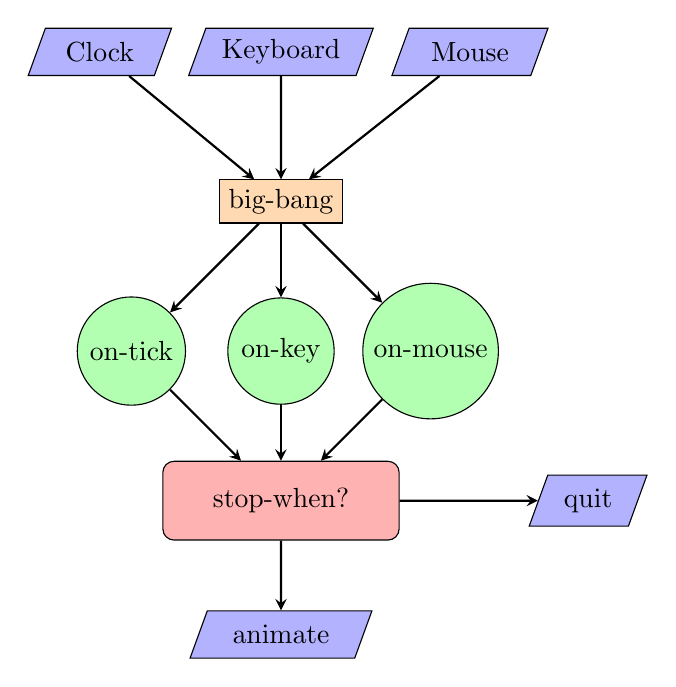
\begin{tikzpicture}[node distance=1.9cm]
      % \node (start) [startstop] {Start};
      \node (in1) [io] {Keyboard};
      \node (in2) [io, right of = in1, xshift=0.5cm] {Mouse};
      \node (in3) [io, left of = in1, xshift=-0.4cm] {Clock};

      \node (pro1) [process, below of=in1] {big-bang};
      % \node (pro2) [process, right of=pro1] {f2};

      \node (dec1) [decision, below of=pro1] {on-key};
      \node (dec2) [decision, right of = dec1] {on-mouse};
      \node (dec3) [decision, left of = dec1] {on-tick};

      \node (out1) [startstop, below of=dec1] {stop-when?};
      \node (out2) [io, below of=out1, yshift=0.2cm] {animate};
      \node (out3) [io, right of=out1, xshift=2cm] {quit};
      % \node (pro3) [process, right of=pro2] {...};
      % \node (out1) [io, right of=pro3] {Output};
      \draw [arrow] (in1) -- (pro1);
      \draw [arrow] (in2) -- (pro1);
      \draw [arrow] (in3) -- (pro1);

      \draw [arrow] (pro1) -- (dec1);
      \draw [arrow] (pro1) -- (dec2);
      \draw [arrow] (pro1) -- (dec3);
      
      \draw [arrow] (dec1) -- (out1);
      \draw [arrow] (dec2) -- (out1);
      \draw [arrow] (dec3) -- (out1);

      \draw [arrow] (out1) -- (out2);
      \draw [arrow] (out1) -- (out3);
    \end{tikzpicture}
  \end{center}
\end{frame}

\begin{frame}
  \frametitle{Our First Event Driven Program}
  With the big bang structure in mind, we can start writing our first big-bang
  program in Racket. It'll draw a square that starts by taking up the whole
  window and will shrink until it disappears.

  \begin{itemize}
  \item<2-> To start with this, we need a function
    that draws a square based on a numerical input.
  \item<3-> \mintinline{Scheme}{(define (number->square s) (square s "solid" "red")}
  \item<4-> In order to animate the square shrinking, we want to continually
    call \mintinline{Scheme}{number->square} with smaller values.
  \end{itemize}

\end{frame}
\end{document}

